\documentclass[runningheads]{llncs}
\title{Erratum: A High-Order Discontinuous Galerkin Solver with Dynamic Adaptive Mesh Refinement to Simulate Cloud Formation Processes }
\titlerunning{A High-Order DG Solver to Simulate Cloud Formation Processes}
\author{Lukas Krenz\orcidID{0000-0001-6378-0778} \and Leonhard Rannabauer \and Michael Bader}
\authorrunning{L.\ Krenz, L.\ Rannabauer, M.\ Bader}
\institute{Department of Informatics, Technical University of Munich\\
  \email{lukas.krenz@in.tum.de}, \email{rannabau@in.tum.de}, \email{bader@in.tum.de}
} 
\usepackage[utf8]{inputenc}
%\usepackage[T1]{fontenc}
\usepackage[american]{babel}
\usepackage[autostyle, english = american]{csquotes}
% \usepackage[%
%   backend=biber,
%   url=false,
%   doi=false,
%   % style=alphabetic,
%   % backref=true,
%   % hyperref=true,
%   maxnames=3,
%   % minnames=3,
%   % maxbibnames=99,
%   firstinits=true,
%   % uniquename=init
%   ]{biblatex}
% \addbibresource{../bibliography.bib}
\usepackage{cite}
\usepackage{todonotes}


\usepackage{caption}
\usepackage{subcaption}
\usepackage{xparse} % for NewDocumentCommand
\usepackage{etoolbox} % for notblank (brackets only when argument)
\usepackage{xstring} % for \IfSubStr
\usepackage{xpatch}
\usepackage{xcolor}
\usepackage{amsmath}
\usepackage{amsfonts}
\usepackage{amssymb}
\usepackage{mathtools} % for \mathclap
\usepackage{nicefrac}
\usepackage{physics} % for derivatives
\usepackage{varioref}
\usepackage{nicefrac}
\usepackage{physics} % for derivatives
\usepackage[separate-uncertainty]{siunitx}
\usepackage{hyperref}
\usepackage[capitalise]{cleveref}
\newcommand{\creflastconjunction}{, and\nobreakspace} % use Oxford comma
\usepackage{graphicx}
\usepackage{multimedia}
%\graphicspath{{../figures/}}
\graphicspath{{.}}
\let\boundary\undefined%
\crefformat{equation}{\eqA{}Eq.~\eqB #2#1#3)}
\crefmultiformat{equation}{Eqs.~\eqMultiA#2#1#3\eqMultiB}%
{ and \eqMultiA#2#1#3\eqMultiB}{, \eqMultiA#2#1#3\eqMultiB}{ and~\eqMultiA#2#1#3\eqMultiB}
\newcommand{\eqA}{}
\newcommand{\eqB}{(}
\newcommand{\eqMultiA}{(}
\newcommand{\eqMultiB}{)}
\DeclareRobustCommand{\pcrefSingle}[1]{%
\begingroup%
  \renewcommand{\eqA}{(}\renewcommand{\eqB}{}%
\cref{#1}%
\endgroup%
}
\DeclareRobustCommand{\pcrefMulti}[1]{%
\begingroup%
    \renewcommand{\eqMultiA}{}\renewcommand{\eqMultiB}{}%
    (\cref{#1})%
\endgroup%
}
\DeclareRobustCommand{\pcref}[1]{%
\IfSubStr{#1}{,}{\pcrefMulti{#1}}{\pcrefSingle{#1}}%
}

\usepackage{bm}
% Commands/Macros
\newcommand{\muscl}{\textsc{muscl}-Hancock}
\newcommand{\dg}{\textsc{dg}}
\newcommand{\ader}{\textsc{ader}}
\newcommand{\aderdg}{\textsc{ader-dg}}
\newcommand{\amr}{\textsc{amr}}
\newcommand{\pde}{\textsc{pde}}
\newcommand{\tbb}{\textsc{tbb}}
\newcommand{\mpi}{\textsc{mpi}}

\newcommand{\softwareName}[1]{#1}
\newcommand{\exahype}{\softwareName{ExaHyPE}}
\newcommand{\exahypeengine}{\softwareName{ExaHyPE Engine}}

% Variables and other equation stuff
\newcommand{\Q}{\bm{Q}}
\newcommand{\gradQ}{\gradient{\Q}}
\newcommand{\Qrho}{\rho}
\newcommand{\Qj}{\rho \bm{v}}
\newcommand{\Qv}{\bm{v}}
\newcommand{\QE}{\rho E}
\newcommand{\potT}{\theta}
\newcommand{\backgroundPotT}{\overline{\theta}}
\newcommand{\pertubationPotT}{\theta'}
\newcommand{\stressT}{\bm{\sigma}}
\newcommand{\pressure}{p}

% Cells
\newcommand{\cell}[1][]{C_{#1}}

% Bold if no index is supplied.
\newcommand{\bmempty}[2]{
\notblank{#2}{#1}{\bm{#1}}
}

% Equation parts
\newcommand{\flux}{\bm{F}}
\newcommand{\viscFlux}{\flux^{v}}
\newcommand{\hyperFlux}{\flux^{h}}
%\newcommand{\source}{\bm{S}}
\newcommand{\source}[1][]{
  \notblank{#1}{
S_{#1}
}{
\bm{S}
}
}
\newcommand{\intdcell}[1]{\int_{\cell} #1 \dd{\bm{x}}}
\newcommand{\tv}{\operatorname{TV}}

\begin{document}
\maketitle 
\begin{abstract}

\keywords{\aderdg{}  \and Navier-Stokes \and Adaptive Mesh Refinement}
\end{abstract}

\todo[inline]{Make clearer, which sections which scenario corresponds to.}
\todo[inline]{Maybe use same figure naming as in original paper.}
%\subsection{Erratum}
\paragraph{Background}
This is an erratum for \cite{krenz2019high}.
\todo[inline]{Zu verklausuliert:}
When trying to reproduce the results, we noticed that we erronously computed the cloud scenarios with a different background pressure and viscosity as stated in the paper.
\todo[inline]{Mention concrete parameters later}
As the former may result in different physical results, we here evaluate the simulations with the correct background pressure of $\SI{100 000 }{\pascal}$.
\todo[inline]{Make clearer that viscosity is both physical and stabilizing}
In our paper, while viscosity follows the Navier-Stokes equations, we use it additionally to stabilize the simulation.
Neither classical CFD scenarios (Taylor-Green, Lid-driven cavity, 3D scenario) nor the convergence test are affected by this.
We recomputed the key cloud scenarios with correct background pressure.
All 2D scenarios were ran with a viscosity of $\mu=0.1$, the 3D scenario required a viscosity of $\mu=0.4$.

\begin{figure}[htb]
  \begin{subfigure}[t]{0.45\columnwidth}
  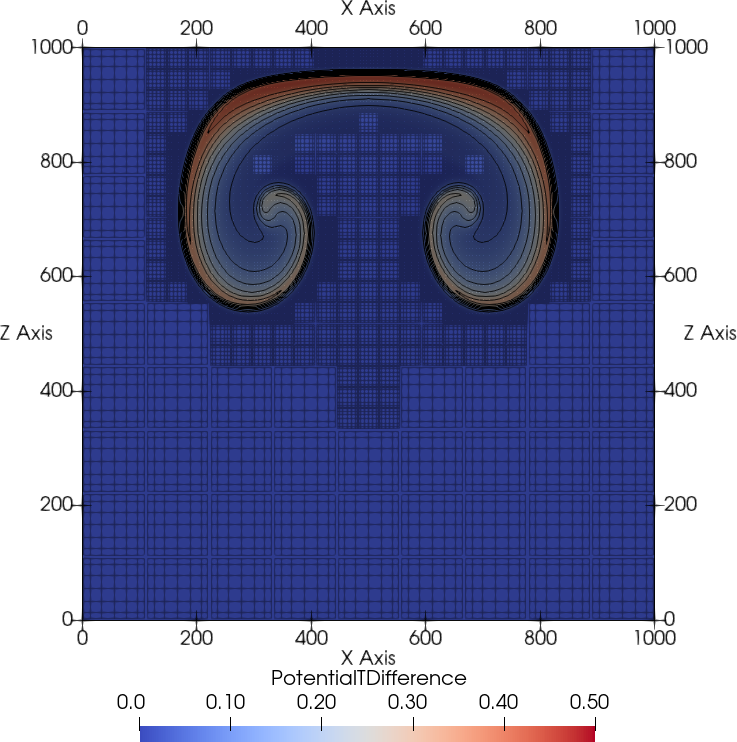
\includegraphics[width=\textwidth]{screenshots/cosine_bubble_2d_dg.png}
  \caption{\label{fig:cosine-bubble-2d-dg-amr}%
  2D Cosine bubble with AMR, computed by ADER-DG method.
  Contours are at $-0.05, 0.05, \ldots 0.45$.
  }
  \end{subfigure}\quad
  \begin{subfigure}[t]{0.45\columnwidth}
  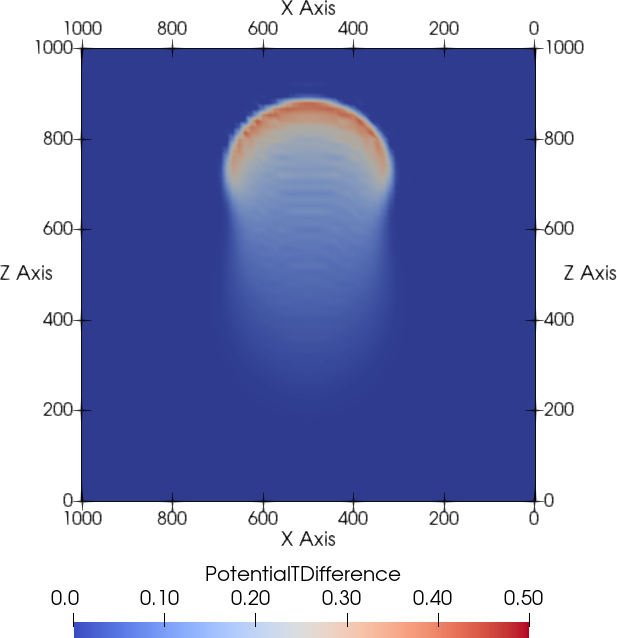
\includegraphics[width=1\textwidth]{screenshots/cosine_bubble_3d_dg.png}
  \caption{\label{fig:cosine-bubble-3d-dg-noamr}%
  3D Cosine bubble without AMR, computed by ADER-DG method.}
  \end{subfigure}
\caption{
  This corresponds to figure 6 of the original paper.
}
\end{figure}
% Settings: visc 0.1, refine: 1.5, coarse: -0.5
\paragraph{Cosine Bubble}
The first scenario is the cosine bubble scenario with and without adaptive mesh refinement (AMR).
We ran it as described in the paper but with the correct background pressure. 
%TODO Refinement settings.
The new result (\cref{fig:cosine-bubble-2d-dg-amr}) shows an excellent agreement with the original results.
The adapted mesh of shows slight differences in the refinement; however, the refinement has the same quality as the original one.
The third scenario is the three-dimensional cosine bubble.
The results, as shown in \cref{fig:cosine-bubble-3d-dg-noamr} are similar to our original results.

\begin{figure}[tb] 
  \centering 
  % or .473 size each, and \\quad inbetween 
    \begin{minipage}[t]{.473\textwidth} 
      \centering 
  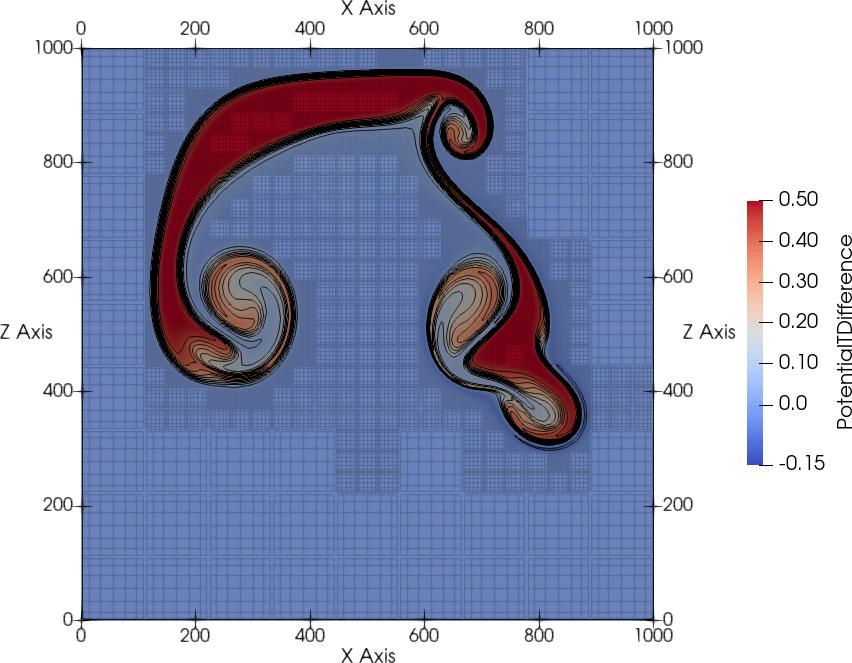
\includegraphics[width=\textwidth]{screenshots/two_bubbles_dg.png}
      %\caption{\label{fig:cavity-flow}Our approximation (solid lines) of the lid-driven cavity flow vs.\ reference solution (crosses) of~\cite{ghia1982high}. 
      %The respective other coordinate is held constant at a value of 0.} 
  \caption{\label{fig:two-bubbles-2d-dg-amr}%
  This corresponds to figure 5 in the original paper.
  2D colliding bubble with AMR, computed by ADER-DG method.
  Contours are at $-0.05, 0.05, \ldots 0.45$.
  }

    \end{minipage}\quad% 
  \begin{minipage}[t]{.473\textwidth}
    \centering
  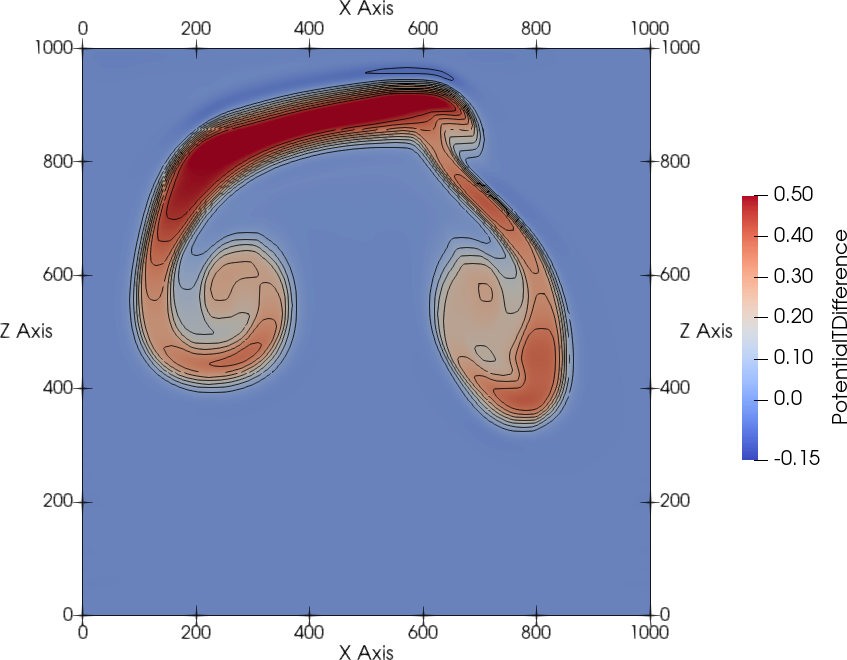
\includegraphics[width=1\textwidth]{screenshots/two_bubbles_fv.png}
  \captionof{figure}{\label{fig:two-bubbles-2d-fv-noamr}%
  This corresponds to figure 4 in the original paper.
  2D colliding bubbles scenario, without AMR, computed with finite volume method.}

  \end{minipage}
  \end{figure}

\paragraph{Colliding Bubble}
The final scenario is the colliding bubble scenario.
We ran this first with the ADER-DG method and a viscosity of $\mu=0.1$.
Similarly to the cosine bubble, the results (\cref{fig:two-bubbles-2d-dg-amr}) show an excellent agreement with the original results (with some small differences in the refinement).
We ran this first with the Finite Volume method using a viscosity of $\mu=0.0$.
The results (\cref{fig:two-bubbles-2d-fv-noamr}) agree with the original results.
% Settings: visc: 0.1, refine: 1.5, coarse: -0.5

To summarize, we reran the affected simulations with the correct background pressure.
After adapting the viscosity, the new results agree well with the original results.

\subsection*{Acknowledgments}
This work was funded by the European Union’s Horizon 2020 Research and Innovation Programme under grant agreements 
No~671698 (project ExaHyPE, \url{www.exahype.eu}) and 
No~823844 (ChEESE centre of excellence, \url{www.cheese-coe.eu}).
Computing resources were provided by the Leibniz Supercomputing Centre (project pr83no).

\bibliographystyle{CP032_spmpsci}
\bibliography{CP032_bibliography}{}
\end{document}
